\section{Photoproduction with linearly polarized beam}%
\label{sec:photoprod}

\subsection{Moment decomposition}%
\label{sec:photoprod:moment}

Systems of two distinguishable spinless particles can also be produced
in photo-production reactions using stationary proton targets.  As in
the case of diffractive reactions discussed in \cref{sec:diffraction},
we are interested in the intermediate meson resonances~$X$ that are
produced in these reactions and that decay into the observed
two-(pseudo)scalar system.  A typical example for such a process is
the reaction
\begin{equation}
  \gamma\, p \to X^0\, p \to \etaOrPr\pi^0\, p,
\end{equation}
which is shown in \cref{fig:photoprod_etaprimepi}.  How to analyze
these reactions was studied in detail by the JPAC collaboration
in~\refsCite{Mathieu:2019fts,Mathieu:2019gxo}.  We will follow these
references here and will derive some equations.

\begin{figure}[bp]
  \centering%
  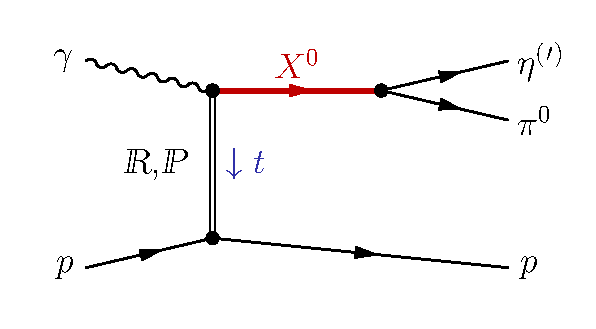
\includegraphics[width=0.5\textwidth]{photoproduction_x_etaprimepi_p}%
  \caption{Scattering of a real photon off a target proton mediated by
  Reggeon exchange.  In this photoproduction process, an intermediate
  state~$X^0$ with well-defined quantum numbers is produced, which in
  the example given here decays into the \etaOrPrPim channel.
  (\Confer~\cref{fig:diffractive_etaprimepi}.)}%
  \label{fig:photoprod_etaprimepi}%
\end{figure}

The analysis is based on the measured intensity distribution, \ie the
number density of events, which is decomposed into partial-wave
amplitudes analogous to the diffractive case in
\cref{eq:diffraction_intensity}:\footnote{\label{fn:photoprod_ampl_redef}This
corresponds to Eq.~(A3) in \refCite{Mathieu:2019fts} with the
phase-space factor~$\kappa$ absorbed into the partial-wave amplitudes,
\ie with the redefinition $\mathcal{T} \to \mathcal{T} /
\sqrt{\kappa}$ (see also footnote~6 in \refCite{Mathieu:2019fts}), and
with Eq.~(A5) inserted.}\todo{Can we express this as
$\abs{\text{amplitude}}^2$?}
\begin{equation}
  \label{eq:photoprod_intensity}
  \mathcal{I}(\Omega, \Phi; w, t)
  = \frac{\dif{N}}{\dif{w}\, \dif{t}\, \dif{\Omega}\, \dif{\Phi}}
  = \sum_{\substack{\ell m \\ \ell' m'}}^\infty
  Y_\ell^m(\Omega)~
  \dUnderbrace{\sum_{\substack{\lambda = \pm 1 \\ \mathclap{\lambda_1, \lambda_2 = \pm 1/2}}}
  \mathcal{T}^\ell_{\!m\, \lambda; \lambda_1\, \lambda_2}(w, t)\,
  \varrho^\gamma_{\lambda\, \lambda'}(\Phi)\,
  \mathcal{T}^{\ell' *}_{\!m'\, \lambda'; \lambda_1\, \lambda_2}(w, t)}{\equiv \varrho^{\ell\, \ell'}_{m\, m'}(w, t, \Phi)}~
  Y_{\ell'}^{m' *}(\Omega).
\end{equation}
Here, $N$~is the (acceptance-corrected) number of measured events,
$w$~is the invariant mass of the two-(pseudo)scalar system, $t$~is the
squared four-momentum transferred from the beam to the target
particle, $\Omega = (\theta, \phi)$ is the direction of one of the two
(pseudo)scalar mesons the~$X$ decays into, measured in the
Gottfried-Jackson or helicity rest frame of~$X$, and~$\Phi$ is the
azimuthal angle between the polarization vector of the linearly
polarized photon and the reaction plane in the $X$~rest frame.  The
$\mathcal{T}^\ell_{\!m\, \lambda; \lambda_1\, \lambda_2}(w, t)$ are
the partial-wave amplitudes that correspond to an intermediate state
with a spin, which is given by the relative orbital angular
momentum~$\ell$ between the two-(pseudo)scalar mesons, and a spin
projection~$m$ \wrt the chosen quantization axis (Gottfried-Jackson
frame: beam direction; helicity frame: momentum direction of~$X$).
This intermediate state is produced in the interaction of a photon
with helicity~$\lambda = \pm 1$ and a target proton with
helicity~$\lambda_1 = \pm 1/2$; the recoil proton has
helicity~$\lambda_2 = \pm 1/2$.  The angular distribution of the
$X$~decay products is given by the spherical harmonics
$Y_\ell^m(\Omega)$~\cite{wikipedia:sphericalHarm} and the dependence
on the polarization angle~$\Phi$ is given by the photon spin-density
matrix~$\mat{\upvarrho}^\gamma(\Phi)$.  In
\cref{eq:photoprod_intensity}, $\varrho^{\ell\, \ell'}_{m\, m'}(w, t,
\Phi)$ is the spin-density matrix element of~$X$ defined analogously
to the diffractive case in \cref{eq:diffraction_spin_dens_def}.

Using the fact that the three Pauli matrices $\vec{\mat{\upsigma}} =
(\mat{\upsigma}_1, \mat{\upsigma}_2, \mat{\upsigma}_3)^T$ and
$\mat{I}_{2 \times 2}$ form a complete set in the space of Hermitian
$2 \times 2$ matrices, we can expand $\mat{\upvarrho}^\gamma(\Phi)$,
\ie
\begin{equation}
  \mat{\upvarrho}^\gamma(\Phi)
  = \frac{1}{2}\, \mat{I}_{2 \times 2} + \frac{1}{2}\, \vec{P}_\gamma(\Phi) \cdot \vec{\mat{\upsigma}}.
\end{equation}
Here, the vector $\vec{P}_\gamma(\Phi)$ describes the photon
polarization.  Its length~$0 \leq P_\gamma \leq 1$ is the degree of
polarization and its direction depends on the kind of
polarization:\footnote{See Eq.~(19) in \refCite{Schilling:1969um}.}
\begin{equation}
  \vec{P}_\gamma(\Phi)
  = \begin{cases*}
    P_\gamma\, (0, 0, \lambda)^T                & for circularly polarized photons with $\lambda = \pm 1$, \\
    -P_\gamma\, (\cos(2 \Phi), \sin(2 \Phi), 0)^T & for linearly polarized photons with polarization angle~$\Phi$.
  \end{cases*}
\end{equation}
Hence, for linearly polarized photons, the intensity distribution in
\cref{eq:photoprod_intensity} can be written as the sum of three
terms:\footnote{See Eq.~(B4) in \refCite{Mathieu:2019fts}.}
\begin{equation}
  \label{eq:photoprod_intensity_sum}
  \mathcal{I}(\Omega, \Phi; w, t)
  = \mathcal{I}_0(\Omega; w, t)
  - \mathcal{I}_1(\Omega; w, t)\, P_\gamma\, \cos(2 \Phi)
  - \mathcal{I}_2(\Omega; w, t)\, P_\gamma\, \sin(2 \Phi)
\end{equation}
with the intensity components
\begin{equation}
  \label{eq:photoprod_intensity_components}
  \mathcal{I}_i(\Omega; w, t)
  = \sum_{\substack{\ell m \\ \ell' m'}}^\infty
  Y_\ell^m(\Omega)\,
  \prescript{i}{}{\varrho}^{\ell\, \ell'}_{m\, m'}(w, t)\,
  Y_{\ell'}^{m' *}(\Omega);
  \quad i = 0, 1, 2
\end{equation}
and the spin-density matrix components\footnote{See Eq.~(11) in
\refCite{Mathieu:2019fts}.}
\begin{align}
  \label{eq:photoprod_rho_0}
  \prescript{0}{}{\varrho}^{\ell\, \ell'}_{m\, m'}(w, t)
  ={}& \frac{1}{2}\quad \sum_{\substack{\lambda = \pm 1 \\ \mathclap{\lambda_1, \lambda_2 = \pm 1/2}}}
  \mathcal{T}^\ell_{\!m\, \lambda; \lambda_1\, \lambda_2}(w, t)\,
  \mathcal{T}^{\ell' *}_{\!m'\, \lambda; \lambda_1\, \lambda_2}(w, t)
  \\
  \label{eq:photoprod_rho_1}
  \prescript{1}{}{\varrho}^{\ell\, \ell'}_{m\, m'}(w, t)
  ={}& \frac{1}{2}\quad \sum_{\substack{\lambda = \pm 1 \\ \mathclap{\lambda_1, \lambda_2 = \pm 1/2}}}
  \mathcal{T}^\ell_{\!m\, {-\lambda}; \lambda_1\, \lambda_2}(w, t)\,
  \mathcal{T}^{\ell' *}_{\!m'\, \lambda; \lambda_1\, \lambda_2}(w, t)
  \\
  \label{eq:photoprod_rho_2}
  \prescript{2}{}{\varrho}^{\ell\, \ell'}_{m\, m'}(w, t)
  ={}& \frac{\imag}{2}\quad \sum_{\substack{\lambda = \pm 1 \\ \mathclap{\lambda_1, \lambda_2 = \pm 1/2}}}
  \lambda\,
  \mathcal{T}^\ell_{\!m\, {-\lambda}; \lambda_1\, \lambda_2}(w, t)\,
  \mathcal{T}^{\ell' *}_{\!m'\, \lambda; \lambda_1\, \lambda_2}(w, t).
\end{align}
Using the above, the spin-density matrix elements of~$X$ in
\cref{eq:photoprod_intensity} are given by
\begin{equation}
  \label{eq:photoprod_spin_dens_sum}
  \varrho^{\ell\, \ell'}_{m\, m'}(w, t, \Phi)
  = \prescript{0}{}{\varrho}^{\ell\, \ell'}_{m\, m'}(w, t)
  - \prescript{1}{}{\varrho}^{\ell\, \ell'}_{m\, m'}(w, t)\, P_\gamma\, \cos(2 \Phi)
  - \prescript{2}{}{\varrho}^{\ell\, \ell'}_{m\, m'}(w, t)\, P_\gamma\, \sin(2 \Phi).
\end{equation}

Note that in \cref{eq:photoprod_intensity_sum}, the $\Phi$~dependence
is separated, \ie neither the $\mathcal{I}_i$ nor the
$\prescript{i}{}{\varrho}^{\ell\, \ell'}_{m\, m'}$ depend on~$\Phi$.
The three intensity components $\mathcal{I}_i(\Omega; w, t)$ (as well
as the three spin-density matrix components in
\cref{eq:photoprod_spin_dens_sum}) are modulated by different
$\Phi$~dependences.  $\mathcal{I}_0(\Omega; w, t)$ is the unpolarized
intensity and is not modulated in~$\Phi$.  As will be shown in the
sections below, $\mathcal{I}_0(\Omega; w, t)$ is equivalent to the
intensity for the diffractive case in \cref{eq:diffraction_intensity}.
The other two components $\mathcal{I}_{1, 2}(\Omega; w, t)$ represent
additional information that is accessible in photoproduction with
linearly polarized beam.  They depend on the photon polarization and
are hence modulated by different $\Phi$~dependences.  Note that the
functions $\cBrk[1]{f_0(\Phi), f_1(\Phi), f_2(\Phi)} = \cBrk[1]{1,
\cos(2 \Phi), \sin(2 \Phi)}$ that modulate the intensity components
constitute an orthogonal set of functions, \ie
\begin{equation}
  \label{eq:photoprod_orthogonality_phi}
  \int_{-\pi}^{+\pi}\hspace{-1.2em} \dif{\Phi}\, f_i(\Phi)\, f_j(\Phi)
  = \pi\, (1 + \delta_{i 0})\, \delta_{i j};
  \quad i, j = 0 ,1, 2. 
\end{equation}

Like for the diffractive case, the partial-wave analysis as well as
the moment decomposition are performed in narrow kinematic cells in
the $(w, t)$ plane, assuming that within each cell all quantities are
in good approximation independent of~$w$ and~$t$.  To simplify
notation we hence omit the~$w$ and $t$~dependencies in all formulas
below, \ie the given formulas are valid in a $(w, t)$ cell.

Analogously to the diffractive case in
\cref{eq:diffraction_intensity_moments}, we decompose the intensity in
\cref{eq:photoprod_intensity_sum} into spherical harmonics to obtain
the moments.  Due to the orthogonality of the $\mathcal{I}_i$ terms in
$\Phi$~space, we can decompose each intensity component
separately:\footnote{See Eq.~(A8) in \refCite{Mathieu:2019fts}.}
\begin{align}
  \label{eq:photoprod_intensity_moments_norm_unpol}
  \mathcal{I}_0(\Omega)
  ={}& \sum_{L M}^\infty \sqrt{\frac{2 L + 1}{4 \pi}}\, H_0(L, M)\, Y_L^M(\Omega)
  \\
  \label{eq:photoprod_intensity_moments_norm_pol}
  \mathcal{I}_{1, 2}(\Omega)
  ={}& -\sum_{L M}^\infty \sqrt{\frac{2 L + 1}{4 \pi}}\, H_{1, 2}(L, M)\, Y_L^M(\Omega).
\end{align}
Here, we have used the same normalization as in
\cref{sec:diffraction:moments_norm}.
\Cref{eq:photoprod_intensity_moments_norm_unpol} is equivalent to
\cref{eq:diffraction_intensity_moments_norm}.  The minus sign in
\cref{eq:photoprod_intensity_moments_norm_pol} is introduced in order
to compensate that the respective intensity components contribute
negatively to the intensity distribution in
\cref{eq:photoprod_intensity_sum}.\footnote{\label{fn:photoprod_intensity_sign}The
minus sign also ensures that $H_1(0, 0) \geq 0$ if the wave set
contains only positive-reflectivity waves with $m \geq 0$ (see
\cref{sec:photoprod:reflectivity} and Appendix~D in
\refCite{Mathieu:2019fts}).}

The corresponding moments are
\begin{align}
  \label{eq:photoprod_moment_norm_unpol}
  H_0(L, M)
  ={}& \frac{1}{2 \pi}\, \sqrt{\frac{4 \pi}{2 L + 1}} \int_{4 \pi}\!\!\!\! \dif{\Omega} \int_{-\pi}^{+\pi}\hspace{-1.2em} \dif{\Phi}\,
  \mathcal{I}(\Omega, \Phi)\, Y_L^{M *}(\Omega)
  \\
  \label{eq:photoprod_moments_norm_pol}
  H_{1, 2}(L, M)
  ={}& \frac{1}{\pi P_\gamma}\, \sqrt{\frac{4 \pi}{2 L + 1}} \int_{4 \pi}\!\!\!\! \dif{\Omega} \int_{-\pi}^{+\pi}\hspace{-1.2em} \dif{\Phi}\,
  \mathcal{I}(\Omega, \Phi)\, Y_L^{M *}(\Omega) \times \begin{cases*}
    \cos(2 \Phi) & for $i = 1$, \\
    \sin(2 \Phi) & for $i = 2$.
  \end{cases*}
\end{align}
Here, $H_0(L, M)$ is equivalent to \cref{eq:diffraction_moments_norm}
for the diffractive case.  The two polarized moments $H_{1, 2}(L, M)$
represent orthogonal angular distributions in~$\Phi$ (see
\cref{eq:photoprod_orthogonality_phi}).


\subsection{Relation between moments and partial-wave amplitudes}%
\label{sec:photoprod:moments_pw}

As in the diffractive case (\confer\
\cref{eq:diffraction_moments_pw_norm}), the moments are linear
combinations of the elements of the respective components of the
spin-density matrix of~$X$.  We see this by inserting
\cref{eq:spherical_harm_prod} into
\cref{eq:photoprod_intensity_components} and comparing with
\cref{eq:photoprod_intensity_moments_norm_unpol,eq:photoprod_intensity_moments_norm_pol},
\ie\footnote{See Eq.~(A9) in \refCite{Mathieu:2019fts}.}
\begin{align}
  \label{eq:photoprod_moment_unpol_pw}
  H_0(L, M)
  ={}& \sum_{\substack{\ell m \\ \ell' m'}}^\infty \sqrt{\frac{2 \ell' + 1}{2 \ell + 1}}
  \clebsch{\ell'}{0}{L}{0}{\ell}{0}\, \clebsch{\ell'}{m'}{L}{M}{\ell}{m}\,
  \prescript{0}{}{\varrho}^{\ell\, \ell'}_{m\, m'}
  \\
  \label{eq:photoprod_moments_pol_pw}
  H_{1, 2}(L, M)
  ={}& -\sum_{\substack{\ell m \\ \ell' m'}}^\infty \sqrt{\frac{2 \ell' + 1}{2 \ell + 1}}
  \clebsch{\ell'}{0}{L}{0}{\ell}{0}\, \clebsch{\ell'}{m'}{L}{M}{\ell}{m}\,
  \prescript{1, 2}{}{\varrho}^{\ell\, \ell'}_{m\, m'},
\end{align}
where the $\prescript{i}{}{\varrho}^{\ell\, \ell'}_{m\, m'}$ are given
by \crefrange{eq:photoprod_rho_0}{eq:photoprod_rho_2}.  For given~$(L,
M)$, the Clebsch-Gordan coefficients restrict the sums to those
quantum-number combinations, for which $\ell' + L + \ell =
\text{even}$ (see \cref{eq:ang_mom_sum}), $\abs{\ell' - L} \leq \ell
\leq \ell' + L$, and $m = m' + M$.  This means that if the
partial-wave amplitudes vanish for $\ell, \ell' > \ell_\text{max}$ the
moments~$H_i(L, M)$ will vanish $L > 2 \ell_\text{max}$.


\subsection{Symmetry properties of moments}%
\label{sec:photo_prod:moments_sym}

To derive the symmetry relations for the photoproduction moments we
use the same approach as in \cref{sec:diffraction:moments_sym}.

From the symmetry property of the spherical harmonics in
\cref{eq:spherical_harm_sym} and the definition of the moments in
\cref{eq:photoprod_moment_norm_unpol,eq:photoprod_moments_norm_pol},
we get
\begin{align}
  H_0^*(L, M)
  ={}& (-1)^M\, \frac{1}{2 \pi}\, \sqrt{\frac{4 \pi}{2 L + 1}} \int_{4 \pi}\!\!\!\! \dif{\Omega} \int_{-\pi}^{+\pi}\hspace{-1.2em} \dif{\Phi}\,
  \mathcal{I}(\Omega, \Phi)\, Y_L^{(-M) *}(\Omega) \notag
  \\
  ={}& (-1)^M\, H_0(L, {-M})
  \\
  H_{1, 2}^*(L, M)
  ={}& (-1)^M\, \frac{1}{\pi P_\gamma}\, \sqrt{\frac{4 \pi}{2 L + 1}} \int_{4 \pi}\!\!\!\! \dif{\Omega} \int_{-\pi}^{+\pi}\hspace{-1.2em} \dif{\Phi}\,
  \mathcal{I}(\Omega, \Phi)\, Y_L^{(-M) *}(\Omega) \times \begin{cases*}
    \cos(2 \Phi) & for $i = 1$, \\
    \sin(2 \Phi) & for $i = 2$
  \end{cases*}
  \notag
  \\
  ={}& (-1)^M\, H_{1,2}(L, {-M}),
  \intertext{\ie}
  \label{eq:photoprod_moments_sym_1}
  H_i^*(L, M)
  ={}& (-1)^M\, H_i(L, {-M});
  \quad i = 0, 1, 2,
\end{align}
which is analogous to \cref{eq:diffraction_moment_sym_1}.

Since the formulas for the intensity components in
\cref{eq:photoprod_intensity_moments_norm_unpol,eq:photoprod_intensity_moments_norm_pol}
have---up to overall signs---the same form as
\cref{eq:diffraction_intensity_moments_norm} for the diffractive case,
we can use the same arguments that lead us to
\cref{eq:diffraction_intensity_moments_general}.  Thus, all intensity
components are real-valued and only moments with $M \geq 0$ are
required to calculate them, \ie
\begin{align}
  \label{eq:photoprod_intensity_moments_unpol_general}
  \mathcal{I}_0(\Omega)
  ={}& \sum_{L = 0}^\infty \sqrt{\frac{2 L + 1}{4 \pi}} \sum_{M = 0}^{L} (2 - \delta_{M 0})\, \Re{H_0(L, M)\, Y_L^M(\Omega)}
  \\
  \label{eq:photoprod_intensity_moments_pol_general}
  \mathcal{I}_{1, 2}(\Omega)
  ={}& -\sum_{L = 0}^\infty \sqrt{\frac{2 L + 1}{4 \pi}} \sum_{M = 0}^{L} (2 - \delta_{M 0})\, \Re{H_{1, 2}(L, M)\, Y_L^M(\Omega)}.
\end{align}

Parity conservation and the assumption that $X$~decays into two
daughter particles with identical parity lead to the following
relations for the spin-density matrix components in
\crefrange{eq:photoprod_rho_0}{eq:photoprod_rho_2}:\footnote{See
Eq.~(A15) in \refCite{Mathieu:2019fts}.}
\begin{equation}
  \label{eq:photoprod_spin_dens_parity}
  \prescript{0, 1}{}{\varrho}^{\ell\, \ell'}_{m\, m'}
  = (-1)^{m - m'}\, \varrho^{\ell'\, \ell}_{{-m}\, {-m'}}
  \quad\text{and}\quad
  \prescript{2}{}{\varrho}^{\ell\, \ell'}_{m\, m'}
  = -(-1)^{m - m'}\, \varrho^{\ell'\, \ell}_{{-m}\, {-m'}}.
\end{equation}
The first equations is analogous to
\cref{eq:diffraction_spin_dens_parity}

Using this together with
\cref{eq:photoprod_moment_unpol_pw,eq:photoprod_moments_pol_pw} and the
symmetry property of the Clebsch-Gordan coefficients in
\cref{eq:clebsch_sym2}, we get\footnote{See Eq.~(A16) in
\refCite{Mathieu:2019fts}.}
\begin{align}
  H_{0, 1}(L, -M)
  ={}& \sum_{\substack{\ell m \\ \ell' m'}}^\infty
  \sqrt{\frac{2 \ell' + 1}{2 \ell + 1}}\,
  \clebsch{\ell'}{0}{L}{0}{\ell}{0}\, \clebsch{\ell'}{-m'}{L}{M}{\ell}{-m}\,
  (-1)^{m - m'}\, \prescript{0, 1}{}{\varrho}^{\ell\, \ell'}_{{-m}\, {-m}'} \notag
  \\
  \label{eq:photoprod_moments_01_sym_2}
  \equalUsing{$\mathclap{\substack{\displaystyle{m \to -m} \\ \displaystyle{m' \to -m'}}}$}{}& \quad
  (-1)^M\, H_{0, 1}(L, M)
  \\
  H_2(L, -M)
  ={}& -\sum_{\substack{\ell m \\ \ell' m'}}^\infty
  \sqrt{\frac{2 \ell' + 1}{2 \ell + 1}}\,
  \clebsch{\ell'}{0}{L}{0}{\ell}{0}\, \clebsch{\ell'}{-m'}{L}{M}{\ell}{-m}\,
  (-1)^{m - m'}\, \prescript{2}{}{\varrho}^{\ell\, \ell'}_{{-m}\, {-m}'} \notag
  \\
  \label{eq:photoprod_moment_2_sym_2}
  \equalUsing{$\mathclap{\substack{\displaystyle{m \to -m} \\ \displaystyle{m' \to -m'}}}$}{}& \quad
  -(-1)^M\, H_2(L, M).
\end{align}
In the last steps of each equation, we used that the second
Clebsch-Gordan coefficient enforces $m' - M = m$,\footnote{Therefore,
$(-1)^{m - m'} = (-1)^{m' - m} = (-1)^M$.} rearranged the terms in the
sum, and compared to
\cref{eq:photoprod_moment_unpol_pw,eq:photoprod_moments_pol_pw}.

From
\cref{eq:photoprod_moments_sym_1,eq:photoprod_moments_01_sym_2,eq:photoprod_moment_2_sym_2}
it follows that
\begin{equation}
  \label{eq:photoprodP_moments_real_imag}
  H_{0, 1}^*(L, M)
  = H_{0, 1}(L, M)
  \quad\text{and}\quad
  H_2^*(L, M)
  = -H_2(L, M).
\end{equation}
Hence, all $H_{0, 1}(L, M)$ must be real-valued and all $H_2(L, M)$
must be purely imaginary.  Consequently, from
\cref{eq:photoprod_moment_norm_unpol,eq:photoprod_moments_norm_pol},
we get\footnote{See Eq.~(B6) in \refCite{Mathieu:2019fts}.}
\begin{align}
  \label{eq:photoprod_moment_0_real}
  H(L, M)
  ={}& \frac{1}{2 \pi}\, \sqrt{\frac{4 \pi}{2 L + 1}} \int_{4 \pi}\!\!\!\! \dif{\Omega} \int_{-\pi}^{+\pi}\hspace{-1.2em} \dif{\Phi}\,
  \mathcal{I}(\Omega, \Phi)\, y_L^M(\theta)\, \cos(M\, \phi)
  \\
  \label{eq:photoprod_moment_0_imag}
  0
  ={}& \frac{1}{2 \pi}\, \sqrt{\frac{4 \pi}{2 L + 1}} \int_{4 \pi}\!\!\!\! \dif{\Omega} \int_{-\pi}^{+\pi}\hspace{-1.2em} \dif{\Phi}\,
  \mathcal{I}(\Omega, \Phi)\, y_L^M(\theta)\, \sin(M\, \phi)
  \\
  \label{eq:photoprod_moment_1_real}
  H_1(L, M)
  ={}& \frac{1}{\pi P_\gamma}\, \sqrt{\frac{4 \pi}{2 L + 1}} \int_{4 \pi}\!\!\!\! \dif{\Omega} \int_{-\pi}^{+\pi}\hspace{-1.2em} \dif{\Phi}\,
  \mathcal{I}(\Omega, \Phi)\, y_L^M(\theta)\, \cos(M\, \phi)\, \cos(2 \Phi)
  \\
  \label{eq:photoprod_moment_1_imag}
  0
  ={}& \frac{1}{\pi P_\gamma}\, \sqrt{\frac{4 \pi}{2 L + 1}} \int_{4 \pi}\!\!\!\! \dif{\Omega} \int_{-\pi}^{+\pi}\hspace{-1.2em} \dif{\Phi}\,
  \mathcal{I}(\Omega, \Phi)\, y_L^M(\theta)\, \sin(M\, \phi)\, \cos(2 \Phi)
  \\
  \label{eq:photoprod_moment_2_real}
  0
  ={}& \frac{1}{\pi P_\gamma}\, \sqrt{\frac{4 \pi}{2 L + 1}} \int_{4 \pi}\!\!\!\! \dif{\Omega} \int_{-\pi}^{+\pi}\hspace{-1.2em} \dif{\Phi}\,
  \mathcal{I}(\Omega, \Phi)\, y_L^M(\theta)\, \cos(M\, \phi)\, \sin(2 \Phi)
  \\
  \label{eq:photoprod_moment_2_imag}
  H_2(L, M)
  ={}& -\imag \frac{1}{\pi P_\gamma}\, \sqrt{\frac{4 \pi}{2 L + 1}} \int_{4 \pi}\!\!\!\! \dif{\Omega} \int_{-\pi}^{+\pi}\hspace{-1.2em} \dif{\Phi}\,
  \mathcal{I}(\Omega, \Phi)\, y_L^M(\theta)\, \sin(M\, \phi)\, \sin(2 \Phi)
\end{align}
The first two equations are equivalent to
\cref{eq:diffraction_moments_real,eq:diffraction_moments_imag}.  Note
that since $\sin(M\, \phi) = 0$ for $M = 0$,
\begin{equation}
  \label{eq:photoprod_moment_2_M0}
  H_2(L, 0) = 0
  \quad\forall\; L.
\end{equation}

Analogous to \cref{eq:diffraction_intensity_moments_real} for the
diffractive case, we can rewrite
\cref{,eq:photoprod_intensity_moments_unpol_general,eq:photoprod_intensity_moments_pol_general}
taking into account
\cref{eq:photoprodP_moments_real_imag}:\footnote{See Eq.~(A17) in
\refCite{Mathieu:2019fts}.}
\begin{align}
  \mathcal{I}_0(\Omega)
  ={}& \sum_{L = 0}^\infty \sqrt{\frac{2 L + 1}{4 \pi}} \sum_{M = 0}^{L} (2 - \delta_{M 0})\, H_0(L, M)\, \Re{Y_L^M(\Omega)} \notag
  \\
  \label{eq:photoprod_intensity_0_moments_real}
  ={}& \sum_{L = 0}^\infty \sqrt{\frac{2 L + 1}{4 \pi}} \sum_{M = 0}^{L} (2 - \delta_{M 0})\, H_0(L, M)\, y_L^M(\theta)\, \cos(M\, \phi)
  \\
  \mathcal{I}_1(\Omega)
  ={}& -\sum_{L = 0}^\infty \sqrt{\frac{2 L + 1}{4 \pi}} \sum_{M = 0}^{L} (2 - \delta_{M 0})\, H_1(L, M)\, \Re{Y_L^M(\Omega)} \notag
  \\
  \label{eq:photoprod_intensity_1_moments_real}
  ={}& -\sum_{L = 0}^\infty \sqrt{\frac{2 L + 1}{4 \pi}} \sum_{M = 0}^{L} (2 - \delta_{M 0})\, H_1(L, M)\, y_L^M(\theta)\, \cos(M\, \phi)
  \\
  \mathcal{I}_2(\Omega)
  ={}& \sum_{L = 0}^\infty \sqrt{\frac{2 L + 1}{4 \pi}} \sum_{M = 0}^{L} (2 - \delta_{M 0})\, \Im{H_2(L, M)}\, \Im{Y_L^M(\Omega)} \notag
  \\
  \label{eq:photoprod_intensity_2_moments_imag}
  ={}& -\imag \sum_{L = 0}^\infty \sqrt{\frac{2 L + 1}{4 \pi}} \sum_{M = 0}^{L} (2 - \delta_{M 0})\, H_2(L, M)\, y_L^M(\theta)\, \sin(M\, \phi).
\end{align}
Note that \cref{eq:photoprod_intensity_2_moments_imag} is identical to
the corresponding expression in Eq.~(A17) in
\refCite{Mathieu:2019fts}, if one considers that $H_2(L, 0) = 0$, \ie
including the terms with $M = 0$ leaves the sum unchanged, and that
$\Im{H_2(L, M)} = -\imag H_2(L, M)$ because $H_2(L, M)$ is purely
imaginary (see \cref{eq:photoprod_moment_2_imag}).  Compared to
\refCite{Mathieu:2019fts}, our formulation is more symmetrical \wrt
\cref{eq:photoprod_intensity_0_moments_real,eq:photoprod_intensity_1_moments_real}.


\subsection{Reflectivity basis}%
\label{sec:photoprod:reflectivity}

In Appendix~D of \refCite{Mathieu:2019fts}, the reflectivity basis is
introduced by defining the partial-wave amplitudes\footnote{See
Eq.~(D1) in \refCite{Mathieu:2019fts}.}\footnote{Alternative
approaches to apply the reflectivity basis are discussed in
\refCite{Salgado:2020}.}
\begin{equation}
  \label{eq:photoprod_amplitude_refl}
  \prescript{\refl}{}{\mathcal{T}}^\ell_{\!m; \lambda_1\, \lambda_2}
  \equiv \frac{1}{2}\, \sBrk{\mathcal{T}^\ell_{\!m\, {+1}; \lambda_1\, \lambda_2}
  - \refl\, (-1)^m\, \mathcal{T}^\ell_{\!{-m}\, {-1}; \lambda_1\, \lambda_2}},
\end{equation}
which are linear combinations of partial-wave amplitudes with opposite
photon helicities~$\lambda$ and opposite $X$~spin projection quantum
numbers~$m$, where $m = -\ell, \ldots, +\ell$.  Hence, the
reflectivity quantum number $\refl = \pm$ effectively replaces the
photon helicity $\lambda = \pm 1$ such that the total number of
amplitudes for given~$\ell$ and~$m$ remains unchanged.

Formulating the intensity model in the reflectivity basis has the
advantage that in the high-energy limit at leading order,
\refl~corresponds to the naturality of the spin-parity exchanged in
the scattering process (see Appendices~C and~D in
\refCite{Mathieu:2019fts}).  Another advantage of the reflectivity
basis is that due to parity conservation partial-wave amplitudes with
opposite~\refl do not interfere.\footnote{See Eq.~(D5) in
\refCite{Mathieu:2019fts}.}  Parity conservation also directly relates
partial-wave amplitudes with opposite helicities of the target and the
recoil proton, \ie\footnote{See Eq.~(D3) in
\refCite{Mathieu:2019fts}.}
\begin{equation}
  \label{eq:photoprod_amplitude_parity_refl}
  \prescript{\refl}{}{\mathcal{T}}^\ell_{\!m; {-\lambda_1}\, {-\lambda_2}}
  = \refl\, (-1)^{\lambda_1 - \lambda_2}\, \prescript{\refl}{}{\mathcal{T}}^\ell_{\!m; \lambda_1\, \lambda_2}.
\end{equation}
Therefore, for given~\refl, $\ell$, and~$m$, only two of the four
possible partial-wave amplitudes are independent, namely the proton
spin-flip amplitude\footnote{See Eq.~(D4) in
\refCite{Mathieu:2019fts}.}
\begin{align}
  \prescript{\refl}{}{\mathcal{T}}^\ell_{\!m; {+1}\, {-1}}
  \equiv{}& \sBrk{\ell}^{(\refl)}_{m; 0}
  \intertext{and the proton spin-non-flip amplitude}
  \prescript{\refl}{}{\mathcal{T}}^\ell_{\!m; {+1}\, {+1}}
  \equiv{}& \sBrk{\ell}^{(\refl)}_{m; 1}.\footnotemark
\end{align}
\footnotetext{In general, scattering reactions with a recoil particle
with spin~$J_R$ are described by $2 J_R + 1$ independent amplitudes
$\sBrk{\ell}^{(\refl)}_{m; k}$ with $k = 0, \ldots, 2 J_R$.}%
Furthermore, since parity is conserved the spin-flip and
spin-non-flip amplitudes do not interfere. In the conventional basis,
it would be difficult to incorporate these parity constraints into
\crefrange{eq:photoprod_intensity_components}{eq:photoprod_rho_2}
because parity relates those $\mathcal{T}^\ell_{\!m\, \lambda;
\lambda_1\, \lambda_2}$ that in addition to opposite~$\lambda_1$
and~$\lambda_2$ quantum numbers also have opposite~$m$
and~$\lambda$.\footnote{See Eq.~(A14) in \refCite{Mathieu:2019fts}.}
However, in the reflectivity basis we can simply write\footnote{See
Eq.~(D7) in \refCite{Mathieu:2019fts}.}
\begin{equation}
  \label{eq:photoprod_rho_refl}
  \prescript{i}{}{\varrho}^{\ell\, \ell'}_{m\, m'}
  = \prescript{i}{}{\varrho}^{(+)\, \ell\, \ell'}_{m\, m'} + \prescript{i}{}{\varrho}^{(-)\, \ell\, \ell'}_{m\, m'};
  \quad i = 0, 1, 2
\end{equation}
with\footnote{See Eq.~(D8) in \refCite{Mathieu:2019fts} and
\cref{fn:photoprod_ampl_redef}.}
\begin{align}
  \label{eq:photoprod_rho_0_refl}
  \prescript{0}{}{\varrho}^{(\refl)\, \ell\, \ell'}_{m\, m'}
  ={}& \sum_{k = 0, 1} \rBrk[2]{\sBrk{\ell}^{(\refl)}_{m; k}\, \sBrk{\ell'}^{(\refl) *}_{m'; k}
  + (-1)^{m - m'}\, \sBrk{\ell}^{(\refl)}_{{-m}; k}\, \sBrk{\ell'}^{(\refl) *}_{{-m'}; k}}
  \\
  \label{eq:photoprod_rho_1_refl}
  \prescript{1}{}{\varrho}^{(\refl)\, \ell\, \ell'}_{m\, m'}
  ={}& -\refl \sum_{k = 0, 1}
  \rBrk[2]{(-1)^m\, \sBrk{\ell}^{(\refl)}_{{-m}; k}\, \sBrk{\ell'}^{(\refl) *}_{m'; k}
  + (-1)^{m'}\, \sBrk{\ell}^{(\refl)}_{m; k}\, \sBrk{\ell'}^{(\refl) *}_{{-m'}; k}}
  \\
  \label{eq:photoprod_rho_2_refl}
  \prescript{2}{}{\varrho}^{(\refl)\, \ell\, \ell'}_{m\, m'}
  ={}& -\imag\, \refl \sum_{k = 0, 1}
  \rBrk[2]{(-1)^m\, \sBrk{\ell}^{(\refl)}_{{-m}; k}\, \sBrk{\ell'}^{(\refl) *}_{m'; k}
  - (-1)^{m'}\, \sBrk{\ell}^{(\refl)}_{m; k}\, \sBrk{\ell'}^{(\refl) *}_{{-m'}; k}}.
\end{align}
In \cref{eq:photoprod_rho_refl}, we sum incoherently over~$\refl =
\pm$ and in
\crefrange{eq:photoprod_rho_0_refl}{eq:photoprod_rho_2_refl}, we sum
incoherently over~$k = 0, 1$, \ie the rank of the
$\prescript{i}{}{\varrho}^{(\refl)\, \ell\, \ell'}_{m\, m'}$ is in
general~2.  By inserting \cref{eq:photoprod_rho_refl} into
\cref{eq:photoprod_intensity_components}, we obtain the intensity
components in the reflectivity basis:
\begin{equation}
  \label{eq:photoprod_intensity_components_refl}
  \mathcal{I}_i(\Omega)
  = \sum_{\substack{\ell m \\ \ell' m'}}^\infty
  Y_\ell^m(\Omega)
  \sBrk[3]{\, \sum_{\refl = \pm} \prescript{i}{}{\varrho}^{(\refl)\, \ell\, \ell'}_{m\, m'}}
  Y_{\ell'}^{m' *}(\Omega);
  \quad i = 0, 1, 2
\end{equation}

Note that usually neither the spin of the target proton
nor the one of the recoil proton is measured.  Still, the intensity
distribution obtained by inserting
\crefrange{eq:photoprod_rho_refl}{eq:photoprod_rho_2_refl} into
\cref{eq:photoprod_intensity_components} has two incoherent sectors
indexed by~$k = 0, 1$ as required by parity conservation.  However, in
this case $k$~has no direct physical interpretation anymore, \ie
experimentally we cannot distinguish, which value of~$k$ belongs to
proton spin-flip and which to proton spin-non-flip.  In practice, one
often assumes that either the spin-non-flip or the spin-flip
amplitudes dominate and sets $k = 0$.  This means the partial-wave
amplitudes are all fully coherent and the spin-density matrix
components in
\crefrange{eq:photoprod_rho_0_refl}{eq:photoprod_rho_2_refl} have
rank~1.

We can relate the moments to the partial-wave amplitudes in the
reflectivity basis by inserting
\crefrange{eq:photoprod_rho_0_refl}{eq:photoprod_rho_2_refl} into
\cref{eq:photoprod_moment_unpol_pw,eq:photoprod_moments_pol_pw}:
\begin{align}
  \label{eq:photoprod_moment_0_pw_refl}
  H_0(L, M)
  ={}& \begin{multlined}[t][0.8\columnwidth]
    \sum_{\substack{\ell m \\ \ell' m'}}^\infty \sqrt{\frac{2 \ell' + 1}{2 \ell + 1}}
    \clebsch{\ell'}{0}{L}{0}{\ell}{0}\, \clebsch{\ell'}{m'}{L}{M}{\ell}{m} \\[-2ex]
    \shoveleft{\hfill \times%
      \sum_{\refl = \pm} \sum_{k = 0, 1} \rBrk[2]{\sBrk{\ell}^{(\refl)}_{m; k}\, \sBrk{\ell'}^{(\refl) *}_{m'; k}
      + (-1)^{m - m'}\, \sBrk{\ell}^{(\refl)}_{{-m}; k}\, \sBrk{\ell'}^{(\refl) *}_{{-m'}; k}}
    }
  \end{multlined}
  \\
  \label{eq:photoprod_moment_1_pw_refl}
  H_1(L, M)
  ={}& \begin{multlined}[t][0.8\columnwidth]
    \sum_{\substack{\ell m \\ \ell' m'}}^\infty \sqrt{\frac{2 \ell' + 1}{2 \ell + 1}}
    \clebsch{\ell'}{0}{L}{0}{\ell}{0}\, \clebsch{\ell'}{m'}{L}{M}{\ell}{m} \\[-2ex]
    \shoveleft{\hfill \times%
      \sum_{\refl = \pm} \refl \sum_{k = 0, 1} \rBrk[2]{(-1)^m\, \sBrk{\ell}^{(\refl)}_{{-m}; k}\, \sBrk{\ell'}^{(\refl) *}_{m'; k}
      + (-1)^{m'}\, \sBrk{\ell}^{(\refl)}_{m; k}\, \sBrk{\ell'}^{(\refl) *}_{{-m'}; k}}
    }
  \end{multlined}
  \\
  \label{eq:photoprod_moment_2_pw_refl}
  H_2(L, M)
  ={}& \begin{multlined}[t][0.8\columnwidth]
    \imag \sum_{\substack{\ell m \\ \ell' m'}}^\infty \sqrt{\frac{2 \ell' + 1}{2 \ell + 1}}
    \clebsch{\ell'}{0}{L}{0}{\ell}{0}\, \clebsch{\ell'}{m'}{L}{M}{\ell}{m} \\[-2ex]
    \shoveleft{\hfill \times%
      \sum_{\refl = \pm} \refl \sum_{k = 0, 1} \rBrk[2]{(-1)^m\, \sBrk{\ell}^{(\refl)}_{{-m}; k}\, \sBrk{\ell'}^{(\refl) *}_{m'; k}
      - (-1)^{m'}\, \sBrk{\ell}^{(\refl)}_{m; k}\, \sBrk{\ell'}^{(\refl) *}_{{-m'}; k}}
    }.
  \end{multlined}
\end{align}
It is important to note that each moment is an incoherent sum of
contributions from both reflectivities, \ie the moments do not
separate these contributions.  Also note that in
\cref{eq:photoprod_moment_0_pw_refl} the contributions from the two
reflectivities enter with the same sign, whereas in
\cref{eq:photoprod_moment_1_pw_refl,eq:photoprod_moment_2_pw_refl}
they enter with opposite sign.  Similarly, each moment is an
incoherent sum over~$k$, \ie the moments do not separate spin-flip and
spin-non-flip amplitudes.

From
\cref{eq:photoprod_moment_0_real,eq:photoprod_moment_0_pw_refl,eq:photoprod_moment_1_pw_refl,eq:photoprod_moment_2_pw_refl}
it follows that in particular
\begin{align}
  H_0(0, 0)
  = \frac{1}{2 \pi} \int_{4 \pi}\!\!\!\! \dif{\Omega} \int_{-\pi}^{+\pi}\hspace{-1.2em} \dif{\Phi}\,
  \mathcal{I}(\Omega, \Phi)
  ={}& \sum_{\ell m}^\infty \prescript{0}{}{\varrho}^{\ell\, \ell}_{m\, m}
  = \sum_{\ell m}^\infty \sum_{\refl = \pm} \sum_{k = 0, 1}
  \rBrk[2]{\Abs[1]{\sBrk{\ell}^{(\refl)}_{m; k}}^2 + \Abs[1]{\sBrk{\ell}^{(\refl)}_{{-m}; k}}^2} \notag
  \\
  \label{eq:photoprod_monent_00_refl}
  ={}& 2 \sum_{\ell m}^\infty \sum_{k = 0, 1}
  \rBrk[2]{\Abs[1]{\sBrk{\ell}^{(+)}_{m; k}}^2 + \Abs[1]{\sBrk{\ell}^{(-)}_{m; k}}^2}
  \\
  H_1(0, 0)
  ={}& -\sum_{\ell m}^\infty \prescript{1}{}{\varrho}^{\ell\, \ell}_{m\, m}
  = \sum_{\ell m}^\infty \sum_{\refl = \pm} \refl \sum_{k = 0, 1}
  (-1)^m \rBrk[2]{\sBrk{\ell}^{(\refl)}_{{-m}; k}\, \sBrk{\ell}^{(\refl) *}_{m; k}
  + \sBrk{\ell}^{(\refl)}_{m; k}\, \sBrk{\ell}^{(\refl) *}_{{-m}; k}}
  \\
  H_2(0, 0)
  ={}& -\sum_{\ell m}^\infty \prescript{2}{}{\varrho}^{\ell\, \ell}_{m\, m}
  = \imag \sum_{\ell m}^\infty \sum_{\refl = \pm} \refl \sum_{k = 0, 1}
  (-1)^m \rBrk[2]{\sBrk{\ell}^{(\refl)}_{{-m}; k}\, \sBrk{\ell}^{(\refl) *}_{m; k}
  - \sBrk{\ell}^{(\refl)}_{m; k}\, \sBrk{\ell}^{(\refl) *}_{{-m}; k}}
\end{align}
Like in the diffractive case (\confer\
\cref{eq:diffraction_moment_00_pw,eq:diffraction_moment_00_pw_refl}),
the lowest unpolarized moment $H_0(0, 0)$ is identical to the
intensity integral and the sum of all partial-wave
intensities.\footnote{The factor~2 in the right-hand side of
\cref{eq:photoprod_monent_00_refl} appears because---due to
\cref{eq:photoprod_amplitude_parity_refl}---we replaced four
amplitudes for the various proton helicities by two amplitudes for
proton spin-flip and spin-non-flip.}

We can simplify the equations for $H_1(0, 0)$ and $H_2(0, 0)$ further
by using
\begin{align}
  \sum_{m = -\ell}^{m = +\ell}
  (-1)^m \sBrk{\ell}^{(\refl)}_{m; k}\, \sBrk{\ell}^{(\refl) *}_{{-m}; k}
  ={}& \sum_{m = -\ell}^{m = -1}
  (-1)^m \sBrk{\ell}^{(\refl)}_{m; k}\, \sBrk{\ell}^{(\refl) *}_{{-m}; k}
  + \sBrk{\ell}^{(\refl)}_{0; k}\, \sBrk{\ell}^{(\refl) *}_{0; k}
  + \sum_{m = +1}^{m = +\ell}
  (-1)^m \sBrk{\ell}^{(\refl)}_{m; k}\, \sBrk{\ell}^{(\refl) *}_{{-m}; k} \notag
  \\
  ={}& \Abs[2]{\sBrk{\ell}^{(\refl)}_{0; k}}^2
  + \sum_{m = +1}^{m = +\ell}
  (-1)^m \rBrk[2]{\sBrk{\ell}^{(\refl)}_{m; k}\, \sBrk{\ell}^{(\refl) *}_{{-m}; k} + \sBrk{\ell}^{(\refl) *}_{m; k}\, \sBrk{\ell}^{(\refl)}_{{-m}; k}} \notag
  \\
  ={}& \Abs[2]{\sBrk{\ell}^{(\refl)}_{0; k}}^2
  + 2 \sum_{m = +1}^{m = +\ell}
  (-1)^m \Re[2]{\sBrk{\ell}^{(\refl)}_{m; k}\, \sBrk{\ell}^{(\refl) *}_{{-m}; k}}
  \in \mathbb{R}.
\end{align}
Using the above, we see that
\begin{align}
  H_1(0, 0)
  ={}& \sum_{\refl = \pm} \refl \sum_{k = 0, 1} \sum_{\ell}^\infty
  \rBrk[3]{\Abs[2]{\sBrk{\ell}^{(\refl)}_{0; k}}^2
  + 2 \sum_{m = +1}^{m = +\ell}
  (-1)^m \Re[2]{\sBrk{\ell}^{(\refl)}_{{-m}; k}\, \sBrk{\ell}^{(\refl) *}_{m; k}}
  + \Abs[2]{\sBrk{\ell}^{(\refl)}_{0; k}}^2
  + 2 \sum_{m = +1}^{m = +\ell}
  (-1)^m \Re[2]{\sBrk{\ell}^{(\refl)}_{m; k}\, \sBrk{\ell}^{(\refl) *}_{{-m}; k}}} \notag
  \\
  ={}& 2 \sum_{\refl = \pm} \refl \sum_{k = 0, 1} \sum_{\ell}^\infty
  \rBrk[3]{\Abs[2]{\sBrk{\ell}^{(\refl)}_{0; k}}^2
  + 2 \sum_{m = +1}^{m = +\ell}
  (-1)^m \Re[2]{\sBrk{\ell}^{(\refl)}_{{-m}; k}\, \sBrk{\ell}^{(\refl) *}_{m; k}}}
  \\
  H_2(0, 0)
  ={}& \imag \sum_{\refl = \pm} \refl \sum_{k = 0, 1} \sum_{\ell}^\infty
  \rBrk[3]{\Abs[2]{\sBrk{\ell}^{(\refl)}_{0; k}}^2
  + 2 \sum_{m = +1}^{m = +\ell}
  (-1)^m \Re[2]{\sBrk{\ell}^{(\refl)}_{{-m}; k}\, \sBrk{\ell}^{(\refl) *}_{m; k}}
  - \Abs[2]{\sBrk{\ell}^{(\refl)}_{0; k}}^2
  - 2 \sum_{m = +1}^{m = +\ell}
  (-1)^m \Re[2]{\sBrk{\ell}^{(\refl)}_{m; k}\, \sBrk{\ell}^{(\refl) *}_{{-m}; k}}} \notag
  \\
  ={}& 0.
\end{align}
As mentioned in \cref{fn:photoprod_intensity_sign}, $H_1(0, 0) \geq 0$
if the wave set contains only positive-reflectivity waves with $m \geq
0$.  $H_2(0, 0)$ vanishes as expected from
\cref{eq:photoprod_moment_2_M0}.


\subsection{Calculation of moments from data}%
\label{sec:photoprod:moments_data}

In order to calculate the photoproduction moments from data, we
generalize the approach that we used to calculate the moments in the
case of diffractive scattering discussed in
\cref{sec:diffraction:acceptance_corr}.  We again assume that
resolution effects in the $(\Omega, \Phi)$ angular space are
negligible, \ie that\footnote{\Confer\
\cref{eq:diffraction_int_meas}.}
\begin{equation}
  \label{eq:photoprod_intensity_meas}
  \mathcal{I}_\text{meas}(\Omega, \Phi)
  = \eta(\Omega, \Phi)\, \mathcal{I}(\Omega, \Phi)
  \equalUsing{\cref{eq:photoprod_intensity_sum}} \eta(\Omega, \Phi) \sBrk[2]{\mathcal{I}_0(\Omega)
  - \mathcal{I}_1(\Omega)\, P_\gamma\, \cos(2 \Phi)
  - \mathcal{I}_2(\Omega)\, P_\gamma\, \sin(2 \Phi)},
\end{equation}
where $\eta(\Omega, \Phi)$ describes the detection efficiency.

We obtain the measured moments analogous to
\cref{eq:diffraction_moments_meas} by decomposing
$\mathcal{I}_\text{meas}(\Omega, \Phi)$ into the same three sets of
orthogonal functions in the $(\Omega, \Phi)$ angular space, \ie
\begin{equation}
  Y_L^M(\Omega) \times \begin{cases}
    1 & \\
    \cos(2 \Phi) & \\
    \sin(2 \Phi) &
  \end{cases},
\end{equation}
that we already used to define the physical moments in
\cref{sec:photoprod:moment}.  As a consequence, we get three sets of
measured moments:
\begin{align}
  \label{eq:photoprod_moment_meas_unpol}
  H_0^\text{meas}(L, M)
  ={}& \frac{1}{2 \pi}\, \sqrt{\frac{4 \pi}{2 L + 1}} \int_{4 \pi}\!\!\!\! \dif{\Omega} \int_{-\pi}^{+\pi}\hspace{-1.2em} \dif{\Phi}\,
  \mathcal{I}_\text{meas}(\Omega, \Phi)\, Y_L^{M *}(\Omega)
  \\
  \label{eq:photoprod_moments_meas_pol}
  H_{1, 2}^\text{meas}(L, M)
  ={}& \frac{1}{\pi P_\gamma}\, \sqrt{\frac{4 \pi}{2 L + 1}} \int_{4 \pi}\!\!\!\! \dif{\Omega} \int_{-\pi}^{+\pi}\hspace{-1.2em} \dif{\Phi}\,
  \mathcal{I}_\text{meas}(\Omega, \Phi)\, Y_L^{M *}(\Omega) \times \begin{cases*}
    \cos(2 \Phi) & for $i = 1$, \\
    \sin(2 \Phi) & for $i = 2$.
  \end{cases*}
\end{align}
This is equivalent to
\cref{eq:photoprod_moment_norm_unpol,eq:photoprod_moments_norm_pol}
and the first equation is equivalent to
\cref{eq:diffraction_moments_meas} for the diffractive case.

With the above moments, the intensity can be written as a sum of three
measured intensities, \ie\footnote{We use the same sign convention for
the intensity components as in \cref{eq:photoprod_intensity_sum}.}
\begin{equation}
  \mathcal{I}_\text{meas}(\Omega, \Phi)
  = \mathcal{I}_0^\text{meas}(\Omega) - \mathcal{I}_1^\text{meas}(\Omega, \Phi) - \mathcal{I}_2^\text{meas}(\Omega, \Phi)
\end{equation}
with\footnote{We cannot use
\cref{eq:photoprod_intensity_0_moments_real,eq:photoprod_intensity_1_moments_real,eq:photoprod_intensity_2_moments_imag}
for the measured intensities because of the arguments in
\cref{fn:complex_moment_decomp}.}
\begin{align}
  \mathcal{I}_0^\text{meas}(\Omega)
  ={}& \sum_{L = 0}^\infty \sqrt{\frac{2 L + 1}{4 \pi}} \sum_{M = 0}^{L} (2 - \delta_{M 0})\,
  \Re{H_0^\text{meas}(L, M)\, Y_L^M(\Omega)}
  \\
  \mathcal{I}_{1, 2}^\text{meas}(\Omega, \Phi)
  ={}& -\sum_{L = 0}^\infty \sqrt{\frac{2 L + 1}{4 \pi}} \sum_{M = 0}^{L} (2 - \delta_{M 0})\,
  \Re{H_{1, 2}^\text{meas}(L, M)\, Y_L^M(\Omega)} \times \begin{cases*}
    \cos(2 \Phi) & for $i = 1$, \\
    \sin(2 \Phi) & for $i = 2$.
  \end{cases*}
\end{align}
The first equation is equivalent to
\cref{eq:diffraction_intensity_moments_meas}.  Note that
$\mathcal{I}_0^\text{meas}(\Omega)$ is independent of~$\Phi$.

To relate the measured to the physical moments, we insert
\cref{eq:photoprod_intensity_meas} and the moment decomposition of the
physical intensity components from
\cref{eq:photoprod_intensity_0_moments_real,eq:photoprod_intensity_1_moments_real,eq:photoprod_intensity_2_moments_imag}
into
\cref{eq:photoprod_moment_meas_unpol,eq:photoprod_moments_meas_pol}:
\begin{align}
  H_0^\text{meas}(L, M)
  ={}& \frac{1}{2 \pi}\, \sqrt{\frac{4 \pi}{2 L + 1}} \int_{4 \pi}\!\!\!\! \dif{\Omega} \int_{-\pi}^{+\pi}\hspace{-1.2em} \dif{\Phi}\,
  \eta(\Omega, \Phi) \sBrk[2]{\mathcal{I}_0(\Omega)
  - \mathcal{I}_1(\Omega)\, P_\gamma\, \cos(2 \Phi)
  - \mathcal{I}_2(\Omega)\, P_\gamma\, \sin(2 \Phi)}
  Y_L^{M *}(\Omega) \notag
  \\
  ={}& \sum_{L' = 0}^\infty \sum_{M' = 0}^{L'} \Bigg[
  H_0(L', M')\,
  \rdUnderbrace{\int_{4 \pi}\!\!\!\! \dif{\Omega} \int_{-\pi}^{+\pi}\hspace{-1.2em} \dif{\Phi}\,
  \eta(\Omega, \Phi)\,
  \rdOverbrace{\sqrt{\frac{2 L' + 1}{4 \pi}}\, (2 - \delta_{M' 0})\, y_{L'}^{M'}(\theta)\, \cos(M'\, \phi)\vphantom{\frac{Y_L^M}{\sqrt{L}}}}{\equiv f_{0, L' M'}^\text{phys}(\Omega, \Phi)}\,
  \rdOverbrace{\frac{1}{2 \pi}\, \sqrt{\frac{4 \pi}{2 L + 1}}\, Y_L^{M *}(\Omega)}{\equiv f_{0, L M}^\text{meas}(\Omega, \Phi)}}%
  {\equiv I^\text{acc}_{0 0, L M\, L' M'}} \notag
  \\
  & + H_1(L', M')\,
  \rdUnderbrace{\int_{4 \pi}\!\!\!\! \dif{\Omega} \int_{-\pi}^{+\pi}\hspace{-1.2em} \dif{\Phi}\,
  \eta(\Omega, \Phi)\,
  \rdOverbrace{P_\gamma\, \sqrt{\frac{2 L' + 1}{4 \pi}}\, (2 - \delta_{M' 0})\, y_{L'}^{M'}(\theta)\, \cos(M'\, \phi)\, \cos(2 \Phi)}{\equiv f_{1, L' M'}^\text{phys}(\Omega, \Phi)}\,
  f_{0, L M}^\text{meas}(\Omega, \Phi)}%
  {\equiv I^\text{acc}_{0 1\, L M\, L' M'}} \notag
  \\
  & + H_2(L', M')\,
  \rdUnderbrace{\int_{4 \pi}\!\!\!\! \dif{\Omega} \int_{-\pi}^{+\pi}\hspace{-1.2em} \dif{\Phi}\,
  \eta(\Omega, \Phi)\,
  \rdOverbrace{\imag\, P_\gamma\, \sqrt{\frac{2 L' + 1}{4 \pi}}\, (2 - \delta_{M' 0})\, y_{L'}^{M'}(\theta)\, \sin(M'\, \phi)\, \sin(2 \Phi)}{\equiv f_{2, L' M'}^\text{phys}(\Omega, \Phi)}\,
  f_{0, L M}^\text{meas}(\Omega, \Phi)}%
  {\equiv I^\text{acc}_{0 2\, L M\, L' M'}}\, \Bigg] \notag
  \\
  \label{eq:photoprod_moment_0_meas2}
  ={}& \sum_{j = 0}^2 \sum_{L' = 0}^\infty \sum_{M' = 0}^{L'}
  I^\text{acc}_{0 j\, L M\, L' M'}\, H_j(L', M').
\end{align}
Similarly,
\begin{align}
  H_1^\text{meas}(L, M)
  ={}& \frac{1}{\pi P_\gamma}\, \sqrt{\frac{4 \pi}{2 L + 1}} \int_{4 \pi}\!\!\!\! \dif{\Omega} \int_{-\pi}^{+\pi}\hspace{-1.2em} \dif{\Phi}\,
  \eta(\Omega, \Phi) \sBrk[2]{\mathcal{I}_0(\Omega)
  - \mathcal{I}_1(\Omega)\, P_\gamma\, \cos(2 \Phi)
  - \mathcal{I}_2(\Omega)\, P_\gamma\, \sin(2 \Phi)}\,
  Y_L^{M *}(\Omega)\, \cos(2 \Phi) \notag
  \\
  ={}& \sum_{L' = 0}^\infty \sum_{M' = 0}^{L'} \Bigg[
  H_0(L', M')\,
  \rdUnderbrace{\int_{4 \pi}\!\!\!\! \dif{\Omega} \int_{-\pi}^{+\pi}\hspace{-1.2em} \dif{\Phi}\,
  \eta(\Omega, \Phi)\,
  f_{0, L' M'}^\text{phys}(\Omega, \Phi)\,
  \rdOverbrace{\frac{1}{\pi P_\gamma}\, \sqrt{\frac{4 \pi}{2 L + 1}}\, Y_L^{M *}(\Omega)\, \cos(2 \Phi)}{\equiv f_{1, L M}^\text{meas}(\Omega, \Phi)}}%
  {\equiv I^\text{acc}_{1 0\, L M\, L' M'}} \notag
  \\
  & + H_1(L', M')\,
  \rdUnderbrace{\int_{4 \pi}\!\!\!\! \dif{\Omega} \int_{-\pi}^{+\pi}\hspace{-1.2em} \dif{\Phi}\,
  \eta(\Omega, \Phi)\,
  f_{1, L' M'}^\text{phys}(\Omega, \Phi)\,
  f_{1, L M}^\text{meas}(\Omega, \Phi)}%
  {\equiv I^\text{acc}_{1 1\, L M\, L' M'}} \notag
  \\
  & + H_2(L', M')\,
  \rdUnderbrace{\int_{4 \pi}\!\!\!\! \dif{\Omega} \int_{-\pi}^{+\pi}\hspace{-1.2em} \dif{\Phi}\,
  \eta(\Omega, \Phi)\,
  f_{2, L' M'}^\text{phys}(\Omega, \Phi)\,
  f_{1, L M}^\text{meas}(\Omega, \Phi)}%
  {\equiv I^\text{acc}_{1 2\, L M\, L' M'}}\, \Bigg] \notag
  \\
  \label{eq:photoprod_moment_1_meas2}
  ={}& \sum_{j = 0}^2 \sum_{L' = 0}^\infty \sum_{M' = 0}^{L'}
  I^\text{acc}_{1 j\, L M\, L' M'}\, H_j(L', M')
\end{align}
and
\begin{align}
  H_2^\text{meas}(L, M)
  ={}& \frac{1}{\pi P_\gamma}\, \sqrt{\frac{4 \pi}{2 L + 1}} \int_{4 \pi}\!\!\!\! \dif{\Omega} \int_{-\pi}^{+\pi}\hspace{-1.2em} \dif{\Phi}\,
  \eta(\Omega, \Phi) \sBrk[2]{\mathcal{I}_0(\Omega)
  - \mathcal{I}_1(\Omega)\, P_\gamma\, \cos(2 \Phi)
  - \mathcal{I}_2(\Omega)\, P_\gamma\, \sin(2 \Phi)}\,
  Y_L^{M *}(\Omega)\, \sin(2 \Phi) \notag
  \\
  ={}& \sum_{L' = 0}^\infty \sum_{M' = 0}^{L'} \Bigg[
  H_0(L', M')\,
  \rdUnderbrace{\int_{4 \pi}\!\!\!\! \dif{\Omega} \int_{-\pi}^{+\pi}\hspace{-1.2em} \dif{\Phi}\,
  \eta(\Omega, \Phi)\,
  f_{0, L' M'}^\text{phys}(\Omega, \Phi)\,
  \rdOverbrace{\frac{1}{\pi P_\gamma}\, \sqrt{\frac{4 \pi}{2 L + 1}}\, Y_L^{M *}(\Omega)\, \sin(2 \Phi)}{\equiv f_{2, L M}^\text{meas}(\Omega, \Phi)}}%
  {\equiv I^\text{acc}_{2 0\, L M\, L' M'}} \notag
  \\
  & + H_1(L', M')\,
  \rdUnderbrace{\int_{4 \pi}\!\!\!\! \dif{\Omega} \int_{-\pi}^{+\pi}\hspace{-1.2em} \dif{\Phi}\,
  \eta(\Omega, \Phi)\,
  f_{1, L' M'}^\text{phys}(\Omega, \Phi)\,
  f_{2, L M}^\text{meas}(\Omega, \Phi)}%
  {\equiv I^\text{acc}_{2 1\, L M\, L' M'}} \notag
  \\
  & + H_2(L', M')\,
  \rdUnderbrace{\int_{4 \pi}\!\!\!\! \dif{\Omega} \int_{-\pi}^{+\pi}\hspace{-1.2em} \dif{\Phi}\,
  \eta(\Omega, \Phi)\,
  f_{2, L' M'}^\text{phys}(\Omega, \Phi)\,
  f_{2, L M}^\text{meas}(\Omega, \Phi)}%
  {\equiv I^\text{acc}_{2 2\, L M\, L' M'}}\, \Bigg] \notag
  \\
  \label{eq:photoprod_moment_2_meas2}
  ={}& \sum_{j = 0}^2 \sum_{L' = 0}^\infty \sum_{M' = 0}^{L'}
  I^\text{acc}_{2 j\, L M\, L' M'}\, H_j(L', M').
\end{align}
\Cref{eq:photoprod_moment_0_meas2} is equivalent to
\cref{eq:diffraction_moments_meas2}.

As expected, the detection
efficiency $\eta(\Omega, \Phi)$ mixes all physical moments.  However,
the relation between measured and physical moments is still given by a
linear equation, \ie
\begin{equation}
  \label{eq:photoprod_moments_meas_matrix}
  \vect{H}_\text{meas}
  = \mat{I}^\text{acc}\, \vect{H},
\end{equation}
which is identical to \cref{eq:diffraction_moments_meas_matrix}.  The
differences \wrt the diffractive case lie in the definition of the
moment vectors~$\vect{H}$~and~$\vect{H}_\text{meas}$.  For
photoproduction, we have to replace the scalar moment for each $(L,
M)$ by a column vector of the three photoproduction
moments:\footnote{Alternatively, one could stack the
vectors~$\vect{H}_0$, $\vect{H}_1$, and~$\vect{H}_2$ on top of each
other (and analogously for $\vect{H}_{\text{meas}, i}$).}
\begin{equation}
  \rBrk[0]{\vect{H}}_{L M}
  = \begin{pmatrix}
    H_0(L M) \\
    H_1(L M) \\
    H_2(L M)
  \end{pmatrix}
  \quad\text{and}\quad
  \rBrk[0]{\vect{H}_\text{meas}}_{L M}
  = \begin{pmatrix}
    H^\text{meas}_0(L M) \\
    H^\text{meas}_1(L M) \\
    H^\text{meas}_2(L M)
  \end{pmatrix}.
\end{equation}
Each of the three photoproduction moments has an associated basis
function, \ie
\begin{align}
  \rBrk[0]{\vect{f}^\text{phys}}_{L M}(\Omega, \Phi)
  ={}& \begin{pmatrix}
    f^\text{phys}_{0, L M}(\Omega, \Phi) \\
    f^\text{phys}_{1, L M}(\Omega, \Phi) \\
    f^\text{phys}_{2, L M}(\Omega, \Phi)
  \end{pmatrix}
  = \sqrt{\frac{2 L + 1}{4 \pi}}\, (2 - \delta_{M 0})\, y_L^M(\theta)
  \begin{pmatrix}
    \cos(M\, \phi) \\
    P_\gamma\, \cos(M\, \phi)\, \cos(2 \Phi) \\
    \imag\, P_\gamma\, \sin(M\, \phi)\, \sin(2 \Phi)
  \end{pmatrix}
  \intertext{and}
  \rBrk[0]{\vect{f}^\text{meas}}_{L M}(\Omega, \Phi)
  ={}& \begin{pmatrix}
    f^\text{meas}_{0, L M}(\Omega, \Phi) \\
    f^\text{meas}_{1, L M}(\Omega, \Phi) \\
    f^\text{meas}_{2, L M}(\Omega, \Phi)
  \end{pmatrix}
  = \frac{1}{\pi}\, \sqrt{\frac{4 \pi}{2 L + 1}}\, Y_L^{M *}(\Omega)
  \begin{pmatrix}
    1 / 2 \\
    \cos(2 \Phi) / P_\gamma \\
    \sin(2 \Phi) / P_\gamma
  \end{pmatrix},
\end{align}
as defined in
\Crefrange{eq:photoprod_moment_0_meas2}{eq:photoprod_moment_2_meas2}.
Consequently, the acceptance integral matrix in
\cref{eq:photoprod_moments_meas_matrix} has the form
\begin{equation}
  \label{eq:photoprod_integral_matrix}
  \rBrk[0]{\mat{I}^\text{acc}}_{i j, L M\, L' M'}
  = \int_{4 \pi}\!\!\!\! \dif{\Omega} \int_{-\pi}^{+\pi}\hspace{-1.2em} \dif{\Phi}\,
  \eta(\Omega, \Phi)\,
  f_{i, L M}^\text{meas}(\Omega, \Phi)\,
  f_{j, L' M'}^\text{phys}(\Omega, \Phi).
\end{equation}
Using similar arguments as in
\cref{fn:diffraction_integral_matrix_perfect_det} one can show that
for a perfect detector with $\eta(\Omega, \Phi) = 1$,
$\mat{I}^\text{acc}$ becomes a unit matrix.

As in the diffractive case, $\mat{I}^\text{acc}$~can be approximated
using a Monte Carlo data sample with $N_\text{gen}$~events that are
uniformly distributed in the two-body phase space.\footnote{This means
the events are uniformly distributed in the $(\cos\theta, \phi, \Phi)$
space.}  After passing the Monte Carlo events through the detector
simulation, event reconstruction, and event selection chains,
$N_\text{acc}$~accepted events remain.  From these events, the
acceptance integral matrix is calculated according to
\begin{equation}
  \label{eq:photoporod_integral_matrix}
  \rBrk[0]{\mat{I}^\text{acc}}_{i j, L M\, L' M'}
  \approx \frac{8 \pi^2}{N_\text{gen}} \sum_{k = 1}^{N_\text{acc}}
  f_{i, L M}^\text{meas}(\Omega_k, \Phi_k)\,
  f_{j, L' M'}^\text{phys}(\Omega_k, \Phi_k).
\end{equation}
This is equivalent to \cref{eq:diffraction_integral_matrix}.  Note
that $f^\text{phys}_{2, L 0}(\Omega, \Phi) = 0$, which is equivalent
to \cref{eq:photoprod_moment_2_M0}.  Hence,
$\rBrk[0]{\mat{I}^\text{acc}}_{i j, L M\, L' M'}$ is singular.  To
restore the invertibility of the acceptance integral matrix the rows
and columns that correspond to $f^\text{phys}_{2, L 0}$ and
$f^\text{meas}_{2, L 0}$ need to be removed from $\mat{I}^\text{acc}$.
Likewise, the elements $\rBrk[0]{\hat{\vect{H}}}_{2, L 0}$ and
$\rBrk[0]{\hat{\vect{H}}_\text{meas}}_{2, L 0}$ should be removed from
$\hat{\vect{H}}$ and $\hat{\vect{H}}_\text{meas}$, respectively.

The measured moments are estimated from the data using the same
approach as in \cref{sec:diffraction:estimation_uncert}, \ie by
replacing the integrals in
\cref{eq:photoprod_moment_meas_unpol,eq:photoprod_moments_meas_pol} by
sums over measured events:
\begin{equation}
  \label{eq:photoprod_moments_meas_estimate}
  \rBrk[0]{\hat{\vect{H}}_\text{meas}}_{i, L M}
  = 2 \pi \sum_{k = 1}^{N_\text{meas}} f_{i, L M}^\text{meas}(\Omega_k, \Phi_k).
\end{equation}
Here, we have chosen the factor $2 \pi$ such that
\begin{equation}
  \label{eq:photoprod_norm_00}
  H_0(0, 0)
  = N
  \quad\text{because}\quad
  f_{0, 0 0}^\text{meas}(\Omega, \Phi)
  = \frac{1}{2 \pi}
  = \text{const}.
\end{equation}
This is equivalent to \cref{eq:diffraction_norm_00}.

With the above definitions, we can use the same formalism described in
\cref{sec:diffraction:estimation_uncert} to calculate the
estimates~$\hat{\vect{H}}$ of the physical moments
from~$\hat{\vect{H}}_\text{meas}$ using
\cref{eq:diffraction_phys_moments}\footnote{Doing so, we again assume
that $\mat{I}^\text{acc}$~is invertible.} and to propagate the
uncertainties from~$\hat{\vect{H}}_\text{meas}$ to~$\hat{\vect{H}}$
using \cref{eq:complex_uncert_prop}.  For the uncertainty propagation,
we estimate the Hermitian and the pseudo-covariance matrix for the
measured moments using the sample covariance analogous to
\cref{eq:diffraction_sample_cov_hermit_meas,eq:diffraction_sample_cov_pseudo_meas}:
\begin{align}
  \rBrk[1]{\hat{\covMatSym}_{\!\hat{\vect{H}}_\text{meas}}}_{i, L M; j, L' M'}
  ={}& \cov[2]{\hat{H}_i^\text{meas}(L, M), \hat{H}_j^\text{meas}(L', M')} \notag
  \\
  \label{eq:photoprod_sample_cov_hermit_meas}
  ={}& \frac{4 \pi^2\, N_\text{meas}}{N_\text{meas} - 1} \sum_{k = 1}^{N_\text{meas}}
  \sBrk[2]{f_{i, L M}^\text{meas}(\Omega_k, \Phi_k)   - \Mean{f_{i, L M}^\text{meas}(\Omega, \Phi)}}
  \sBrk[2]{f_{j, L' M'}^\text{meas}(\Omega_k, \Phi_k) - \Mean{f_{j, L' M'}^\text{meas}(\Omega, \Phi)}}^*
  \\
  \rBrk[1]{\hat{\tilde{\covMatSym}}_{\!\hat{\vect{H}}_\text{meas}}}_{i, L M; j, L' M'}
  ={}& \cov[2]{\hat{H}_i^\text{meas}(L, M), \hat{H}_j^{\text{meas}\, *}(L', M')} \notag
  \\
  \label{eq:photoprod_sample_cov_pseudo_meas}
  ={}& \frac{4 \pi^2\, N_\text{meas}}{N_\text{meas} - 1} \sum_{k = 1}^{N_\text{meas}}
  \sBrk[2]{f_{i, L M}^\text{meas}(\Omega_k, \Phi_k)   - \Mean{f_{i, L M}^\text{meas}(\Omega, \Phi)}}
  \sBrk[2]{f_{j, L' M'}^\text{meas}(\Omega_k, \Phi_k) - \Mean{f_{j, L' M'}^\text{meas}(\Omega, \Phi)}}.
\end{align}

\todoInl{Add example}